%------------------------------------------------
\begin{frame}
\frametitle{Equilibrium I}


\begin{columns}[c] % The "c" option specifies centered vertical alignment while the "t" option is used for top vertical alignment
\column{.28\textwidth} % Left column and width
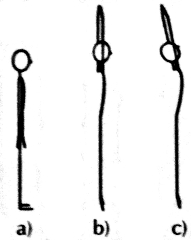
\includegraphics[width=1\linewidth]{Ex1.jpg}
\column{.75\textwidth} % Right column and width
\begin{itemize}
\item[a)] Stand hip--wide and evenly distribute your weight on your feet. Consciously get in \structure{contact with the floor} (gravity), ``\structure{root}'' yourself.

Feel your \structure{crown} and let yourself being ``pulled \structure{upwards}'' (levitation).

Focus on your middle, the hara-centre (below your navel). Feel your \structure{center}, breathe into it.

Imagine a \structure{vertical axis}, from your feet to your crown. \pause
\item[b)] Slowly and carefully \structure{lift yourself} on the tip of your toes. \pause
\item[c)] Slowly direct your \structure{gaze upward}.
\end{itemize}
\end{columns}
\end{frame}
%------------------------------------------------
%------------------------------------------------
\begin{frame}
\frametitle{Equilibrium II}


\begin{columns}[c] % The "c" option specifies centered vertical alignment while the "t" option is used for top vertical alignment
\column{.4\textwidth} % Left column and width
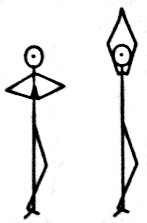
\includegraphics[width=0.8\linewidth]{Ex2.jpg}
\column{.6\textwidth} % Right column and width
First feel your center. Put \structure{one foot on the other}. 

Put your \structure{hands together} in front of you, then \structure{lift them} slowly up; eventually lift your gaze, too.

Breathe very calmly and focus on your center.

Repeat on the other side.
\end{columns}
\end{frame}
%------------------------------------------------
%------------------------------------------------
\begin{frame}
\frametitle{Equilibrium III}


\begin{columns}[c] % The "c" option specifies centered vertical alignment while the "t" option is used for top vertical alignment
\column{.3\textwidth} % Left column and width
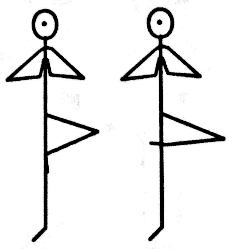
\includegraphics[width=1\linewidth]{Ex3.jpg}
\column{.7\textwidth} % Right column and width
First feel your center. Take one \structure{foot} 
and rest it against the \structure{inner side of your knee}, if possible to your \structure{thigh}.

Hold your hands in front of your sternum.

Breathe calmly. You can close your eyes. Breathe very calmly and focus on your center.

Repeat on the other side.
\end{columns}
\end{frame}
%------------------------------------------------
%------------------------------------------------
\begin{frame}
\frametitle{Equilibrium IV}


\begin{columns}[c] % The "c" option specifies centered vertical alignment while the "t" option is used for top vertical alignment
\column{.3\textwidth} % Left column and width
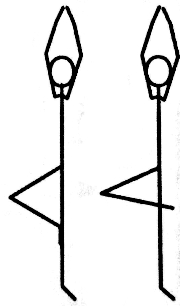
\includegraphics[width=0.8\linewidth]{Ex4.jpg}
\column{.7\textwidth} % Right column and width
The same as before, but this time \structure{raise your hands}. You can close your eyes.

Breathe calmly and focus on your center.

Repeat on the other side.
\end{columns}

\vspace{1cm}
Back to \href{run:./Exercises.pdf}{\underline{exercises}}.

\end{frame}
%------------------------------------------------
